\chapter{Theoretical concepts}

This chapter will go over the most important concepts in the thesis before we apply them in practice in the later chapters. We look at what is usability and how it relates to HCI (human--computer interaction), i.e. software and video games, and what are heuristics in the context of usability. We also provide an overivew of tutorials.

\section{Usability}
Usability is a word that can come up often in conversation. It sounds familiar and should be rather easily explained. However, it is not necessarily that simple in this contex. Is something usable? If we can use something, does that mean that the artifact is usable? How can we measure this? Is there good usability and bad usability? Of course we can just say something is usable, but that does not necessarily tell us anything more than that there exists something we can interact with. To further complicate the issue, usability does not even necessarily mean the end product or the user interface the user will be interacting with; we can also apply usability guidelines to the actual software development processes \cite{Carvajal2013}. Usability also relates closely to design. We can talk about Norman doors -- doors that are so badly designed and unusable that we can't figure out how to open them -- derived from Donald Norman's classic book \textit{The Design of Everyday Things} \cite{Norman2013a}. In this sense usability is just not something that exists, but is required. We can not take it away or separate it from the under-the-hood functionality, or it becomes pointless since we are unable to utilize it. Let us say we have a microwave oven that works perfectly, but we remove all the buttons and displays from the front panel. It is still capable of cooking things, but it is really hard to enable that functionality since we have really poor options for interaction. Perhaps we could screw the whole thing open and try to apply some MacGyverisms and ad hoc solutions in order to produce a warm meal, but that would most likely feel highly unusable. The next step could be that we add one button to the front panel that turns the oven on and off. We would also need a way to open the oven's door. After that all kinds of additional things come to mind that we in a way take for granted. At some point we will start to approach the other end of the usability spectrum: we have too many things and also things that are irrelevant. Things that only come in the way of the core functionality we want to enable or convey. Some might feel that the best kind of microwave would be the one that has only one button to turn it on and off, many might want to be able to change the power and add a timer and other typical things we might have in microwaves. The core issue, however, is that without adding usability to the object, its existence comes in a sense pointless. Taking this idea of usability and bringing it to many different areas in life -- from doors and microwaves to video games and many things in between -- we can start to appreciate the value it gives us in the tools and entertainment we come to contact with in a weekly and even a daily basis. This also brings forth the idea, that no matter what kind of great tools and things we are able to create, they will make no difference unless we think about their usability. Through usability we will strive to increase and maximize the potential of anything we have decided to make.

One classic view on usability comes from Jakob Nielsen in the form of a usability definition and a list of 10 usability heuristics for user interace design. We will look at heuristics more closely in the following chapters. Nielsen defines usability as five quality components \cite{Nielsen2012}:

\begin{itemize}
	\item Learnability: How easy is it for users to accomplish basic tasks the first time they encounter the design?
	\item Efficiency: Once users have learned the design, how quickly can they perform tasks?
	\item Memorability: When users return to the design after a period of not using it, how easily can they reestablish proficiency?
	\item Errors: How many errors do users make, how severe are these errors, and how easily can they recover from the errors?
	\item Satisfaction: How pleasant is it to use the design?
\end{itemize}

Nielsen also mentions a sixth attribute for usability he calls \textit{utility}. It is an important attribute to discern, since utility is at the core of \textit{why} something is made in the first place. We can imagine something that takes into account all the principles of good design and usability, is beautiful in every way and a pleasure to use, but does not really do any or most of the things we need it to or designed it to do. Through this marriage of usability and utility, Nielsen comes to define whether something is actually \textit{useful} \cite{Nielsen2012}: 

\begin{itemize}

	\item Definition of Utility = whether it provides the features you need.
	\item Definition of Usability = how easy and pleasant these features are to use.
	\item Definition of Useful = usability + utility.

\end{itemize}

We also have to keep in mind that here, usability can refer to any type of design and design process, not only something related to software and games. In the following sections, usability is dissected in a more specific context, i.e. how it has been defined in relation to software and video games.

\subsection{Usability in software}
Standards have been created to help with designing usable interfaces for software. Two central standard bodies involved in developing standards for HCI (Human--computer interaction) and usability are International Organization for Standardization (ISO) and International Electrotechnical Commission (IEC). The word \textit{usability} has been summarized in a standard as follows:

\begin{displayquote}

\textit{Usability}: the extent to which a product can be used by specified users to achieve specified goals with effectiveness, efficiency and satisfaction in a specified context of use -- ISO 9241-11: GUIDANCE ON USABILITY (1998) \cite{ISO1998}

\end{displayquote}

Later, we will attempt to draw a line from the mentioned user satisfaction to player satisfaction in games. Standards for HCI and usability are generally categorized as follows \cite{Bevan2006}:
\begin{enumerate}
	\item The use of the product (effectiveness, efficiency and satisfaction in a particular context of use).
	\item The user interface and interaction.
	\item The process used to develop the product.
	\item The capability of an organization to apply user-centered design.
\end{enumerate}

This structure shows us the way in which usability is generated into the use of the product (1) starting from the capability of an organization (4). 

\begin{figure}[h]
	\centering
	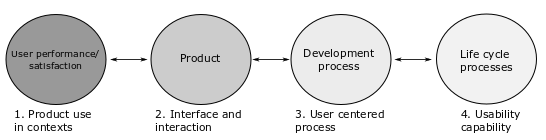
\includegraphics[width=\textwidth]{hci_standards}
	\caption{The logical relationships of standards related to usability \cite{Bevan2006}}
\end{figure}

It is further exemplified in Figure 2.1, illustrating the logical relationships: "the objective is for the product to be effective, efficient and satisfying when used in the intended contexts. A prerequisite for this is an appropriate interface and interaction. This requires a user-centred design process, which to be achieved consistently requires an organizational capability to support user-centred design." \cite{Bevan2006} When we look at ISO 9241-11, there is a promising toolkit for how to take usability into account, specifically considering user performance and satisfaction, but also the context of the system. They claimed that it is also possible to derive factors affecting the quality of the entire system from these variables of user performance and satisfaction. \cite{Bevan2006} Interestingly, this can lead us to think about the quality of video game tutorials, and how they might function as this mediating component between the user (player) and the actual game they are attempting to learn -- or perhaps even more so, are being taught. There have been further definitions of usability as a software engineering standard by ISO and IEC, namely ISO/IEC 9126-1, which defined usability as a set of attributes that bear on the effort needed for use, and on the individual assessment of such use, by a stated or implied set of users. \cite{Bevan2006} This has been later replaced with the ISO/IEC 9126-1 which has a new definition \cite{Bevan2006}:

\begin{displayquote}
	
	\textit{Usability}: the capability of the software product to be understood, learned, used and attractive to the user, when used under specified conditions.
	
\end{displayquote}

This new standard also brought attention to the important aspect of utility, similarly as to how Nielsen has defined it, that in the context of usability there is not necessarily much use to define usability per se, but rather realize how it always operates in a given context and aims to maximize the utility of the underlying capabilities, hence making usability valuable only if the requirements made by the specified conditions are fulfilled. The ISO/IEC 9126-1 also uses another term, \textit{quality in use}, attempting to combine the ideas of usability in general but also the importance of context \cite{Bevan2006}:

\begin{displayquote}
	
	\textit{Quality in use}: the capability of the software product to enable specified users to achieve specified goals with effectiveness, productivity, safety and satisfaction in specified contexts of use.
	
\end{displayquote}

These definitions are bringing us closer to how we can think about usability in the context of video games. Interestingly, with virtual reality (VR) technology currently becoming more widely available, even the safety aspect, originally perhaps geared more towards industry applications, can be a valuable thing to take into account.

\subsection{Usability in video games}

Game developers making games for other game developers and video game enthusiasts at large does not necessarily bring forth the question of usability very early in the process. It is when broader audiences are sought, and perhaps people who have never played games before, when the question becomes more important. \cite{Isbister2008} In the context of usability, the term user satisfaction comes up often. A host of problems can be found in the usability of different video game genres \cite{Pinelle2008b}. The forementioned \textit{effectiveness} and \textit{efficiency} can also be related to games, but being first and foremost a medium for entertainment and storytelling, rather than a tool for solving problems -- i.e. some professional type of software -- it might be important to think about how to achieve player satisfaction first. This is important in part because games are first and foremost a form of entertainment and are acquired voluntarily. A game that is not fun will most likely not be very succesful. \cite{Federoff2002} In this sense, we could think about effectiveness and efficiency as something that can help us deliver satisfaction. That is to say, we create a tutorial that is effective and efficient in teaching the player how to play the game, which brings us to create player satisfaction. There is also an important difference between video games and other types of software: we could say that generally, video games almost always come with an integrated tutorial, whereas most other types of software do not. Why is this? Could it be that games are usually meant to be played in certain predefined ways, and the rest, more or less productive types of software can be used for different tasks depending on the environment? Spreadsheet software, web browsers and other common tools rarely teach you how to use them when first opened. It can be that they have become so commonplace that if guidance is required, it is brought from an outside entity, such as a consultant coming into a company to give training in a specific software. Another thing is that these types of software are generally meant to be used indefinitely, whereas games are completed; the story comes to a close, a character is leveled to the highest possible level, all functionality (character skills etc.) is finally unlocked, every puzzle solved and so on. This means that a tutorial can be created for a set of predefined outcomes and mechanics. Surely there can be a tutorial on how to enter numbers in a spreadsheet, but the possibilities of using those numbers to your advantage are so numerous that creating a tutorial within the software that would show you everything doesn't sound like a justified way to spend resources on.

What, then, is the significance of usability in games? A set of predefined outcomes and/or mechanics is not necessarily a huge platform to build on, which means that creating meaningful and useful tutorials should be easier. This is not to say that all games are simple and easy. It is possible to create a system of numerous possibilities where the player operates with simple mechanics. Since there are so many genres of games, this can often be a case by case problem. Even within a genre, games often like to reinvent the wheel and introduce some type of new gimmicks previously unfamiliar to the genre, to provide a sense of freshness and novelty. It is through these mechanics and the interfaces we use to interact with them we start to create the basis for a need for a tutorial: which mechanics to present and the best way to teach them to a new player.

\section{Heuristics in usability}

So how would we then evaluate a tutorial in a given video game? There are a few possibilities to do this, of which popular are expert review and user or usability testing. Since the aim of this thesis is to provide an expert review solution, we will not be looking at usability testing with a group of users. Rather, we need to build a set of heuristics we can base our evaluation on and then proceed to go through a number of tutorials and see how well they fit within the usability guidelines defined in the heuristics we are going to form. But what is a heuristic? The Merriam-Webster dictionary defines the word heuristic as follows \cite{merriam2007}: 

\begin{itemize}
	\item Involving or serving as an aid to learning, discovery, or problem-solving by experimental and especially trial-and-error methods§ 
	\item Heuristic techniques 
	\item A heuristic assumption; also :  of or relating to exploratory problem-solving techniques that utilize self-educating techniques (such as the evaluation of feedback) to improve performance 
	\item A heuristic computer program 
	
\end{itemize}

This is still a very broad definition and does not necessarily tell us much here. One way is to think of a heuristic as a shortcut or a guideline-based method \cite{Isbister2008}. Heuristics in e.g. psychology stands for shortcuts people use to tackle complex problems with incomplete information \cite{Kahneman1982}. In the context of usability we can think of heuristics as a design guideline that we can use as tools for evaluation, which traditionally relates to user interfaces. The goal here is to make the interface easy to learn, use and master, opposing the usual game design goal of "easy to learn, difficult to master". \cite{Desurvire2004} It's not necessarily a good idea to make the interface difficult to learn, even if gameplay-wise this can often be a good choice. Desurvire et al. further state that we can not only think about games through the interface: we must evaluate other factors as well, such as game play, story and mechanics \cite{Desurvire2004}. In the third chapter we will be looking at these heuristics in more detail. Nielsen and Molich \cite{Nielsen1990} have defined four ways to evaluate a user interface: 

\begin{itemize}
\item Formally by some analysis technique
\item Automatically by a computerized procedure
\item Empirically by experiments with test users 
\item Heuristically by simply looking at the interface and passing judgement according to ones own opinion
\end{itemize}

Now, we don't want to simply look at some games and shout out some opinions based on how we feel like. It would be more useful to base it on some existing heuristics about usability, but usability heuristics for video game tutorials are rare. Therefore, we can find some existing heuristic lists for usability evaluation in general, and combine these lists to better suit the evaluation of video game tutorials. In their paper \textit{Heuristic evaluation of user interfaces} Nielsen and Molich also provide a subset of principles to be used for the evaluation in question: \cite{Nielsen1990}

\begin{itemize}
	\item Simple and natural dialogue
	\item Speak the user's language
	\item Minimize user memory load
	\item Be consistent
	\item Provide feedback
	\item Provide clearly marked exits
	\item Provide shortcuts
	\item Good error messages
	\item Prevent errors
\end{itemize}

At this point these principles serve more as an example to describe what kind of heuristics can be used in a heuristic evaluation. We will have a large pool of different heuristics which we will combine to use in our expert review of tutorials. Some bullet points here might feel self-evident and some might not feel right for the context of video game tutorials, so we must make decisions on whether to include any given heuristics for our analysis in question. Furthermore, such lists are highly valuable for an evaluation, since we don't have to rely on our intuition alone, but have a scientific basis for evaluating different artifacts. Nielsen and Molich have also defined other advantages for using heuristic evaluation: \cite{Nielsen1990}

\begin{itemize}
	\item It is cheap
	\item It is intuitive and it is easy to motivate people to do it
	\item It does not require advanced planning
	\item It can be used early in the development process
\end{itemize}

However, it is not only always positives regarding heuristic evaluation, especially when performed by a single person. It has been concluded that at least in some cases heuristic evaluation would be best done with three to five evaluators separately, and it can also be difficult to come up with solutions to the usability problems found when using a heuristic approach. \cite{Nielsen1990} On the other hand, when we are going to look at video game tutorials, we will have a combination of a number of different heuristics to use, and also games from different genres, to which some forms of heuristics might be better suitable than others. The studies by Nielsen and Molich used in part static screen dumps and old voice response systems using telephone buttons. Those systems are not exactly similar to modern video games, so we can't yet say with certainty how a heuristic approach might work for video game tutorials specifically, even if it hasn't always worked well for other types of systems and interfaces. This could become even more evident when we compare different video game genres and the types of tutorials therein. In that regard, applying a combination of different heuristics to different types of contexts (i.e. video game genres) we can hope to expect many different types of outcomes for the heuristic approach.

\section{The role of the tutorial in a video game}

The word tutorial can be interpreted as the transferring of knowledge. It doesn't necessarily then mean that there would have to be a separate tutorial section in the game, but rather the tutorial can be happening occasionally into many hours in the game, as new mechanics or strategies are introduced.
